\documentclass[10pt,aspectratio=169]{beamer}
\usepackage{amsmath,amssymb,booktabs,array,microtype}
\usepackage{tikz}
\usetikzlibrary{positioning,arrows.meta,calc}
\usepackage{xcolor}

\definecolor{navy}{HTML}{16324F}
\definecolor{teal}{HTML}{148A8A}
\definecolor{gold}{HTML}{E5A823}
\definecolor{brick}{HTML}{A4473A}
\definecolor{lightblue}{HTML}{E9F1F7}
\definecolor{lightgold}{HTML}{FBF4E3}
\definecolor{softgray}{HTML}{F2F4F5}

\setbeamercolor{normal text}{fg=navy,bg=white}
\setbeamercolor{structure}{fg=teal}
\setbeamercolor{frametitle}{fg=white,bg=navy}
\setbeamercolor{title}{fg=white}
\setbeamercolor{subtitle}{fg=white}
\setbeamercolor{author}{fg=white}
\setbeamercolor{date}{fg=white}
\setbeamercolor{block title}{fg=white,bg=teal}
\setbeamercolor{block body}{fg=navy,bg=lightblue}
\setbeamercolor{alertblock title}{fg=white,bg=brick}
\setbeamercolor{alertblock body}{fg=navy,bg=lightgold}
\setbeamercolor{exampleblock title}{fg=white,bg=gold!85!black}
\setbeamercolor{exampleblock body}{fg=navy,bg=lightgold}
\setbeamercolor{footline}{fg=navy,bg=softgray}
\setbeamerfont{frametitle}{series=\bfseries,size=\large}
\setbeamerfont{title}{series=\bfseries,size=\LARGE}
\setbeamerfont{subtitle}{size=\large}
\setbeamertemplate{navigation symbols}{}
\setbeamertemplate{itemize item}{\color{teal}$\blacktriangleright$}
\setbeamertemplate{itemize subitem}{\color{gold}$\bullet$}
\setbeamertemplate{footline}{%
  \leavevmode\hbox{%
    \begin{beamercolorbox}[wd=.82\paperwidth,ht=2.7ex,dp=1.1ex,leftskip=1em]{footline}%
      \insertsectionhead
    \end{beamercolorbox}%
    \begin{beamercolorbox}[wd=.18\paperwidth,ht=2.7ex,dp=1.1ex,center]{footline}%
      \insertframenumber/\inserttotalframenumber
    \end{beamercolorbox}}}

\newcommand{\E}{\mathbb{E}}
\newcommand{\trans}{^{\prime}}
\newcommand{\key}[1]{\textcolor{teal}{\textbf{#1}}}
\newcommand{\caution}[1]{\textcolor{brick}{\textbf{#1}}}
\newcommand{\norm}[1]{\left\lVert#1\right\rVert}

\title{Strategic Investment in a Forward-Looking\\Monetary--Fiscal Markov Game}
\subtitle{Analytical mechanism, equilibrium construction, and parameter regions}
\author{Monetary--Fiscal Coordination Project}
\date{2 October 2026}

\begin{document}

\begin{frame}[plain]
\begin{tikzpicture}[remember picture,overlay]
  \fill[navy] (current page.south west) rectangle (current page.north east);
  \fill[teal] (current page.south west) rectangle ([xshift=0.20\paperwidth]current page.north west);
  \fill[gold] ([yshift=-0.045\paperheight]current page.north west) rectangle
              ([yshift=-0.06\paperheight]current page.north east);
\end{tikzpicture}
\vspace{0.8cm}
\hspace{0.18\textwidth}
\begin{minipage}{0.78\textwidth}
  \maketitle
\end{minipage}
\end{frame}

\section{Purpose and roadmap}

\begin{frame}{Purpose of this deck}
\begin{alertblock}{Single equilibrium concept}
The dynamic model is a \textbf{feedback Markov-perfect equilibrium (MPE)}.
Policy is reset each period as a function of the payoff-relevant state.
\end{alertblock}
\begin{columns}[T,onlytextwidth]
\column{0.47\textwidth}
\begin{block}{What we will do}
\begin{itemize}
  \item derive the static interaction statistic;
  \item show how adjustment costs create a strategic state;
  \item construct the recursive LQ policy game;
  \item embed it in a forward-looking NK private block;
  \item characterize parameter regions analytically.
\end{itemize}
\end{block}
\column{0.47\textwidth}
\begin{exampleblock}{What we will not do}
\begin{itemize}
  \item impose country-specific parameter values;
  \item present data-based impulse responses;
  \item select arbitrary numerical adjustment costs;
  \item infer importance from a strategic share alone.
\end{itemize}
\end{exampleblock}
\end{columns}
\end{frame}

\begin{frame}{Analytical construction}
\centering
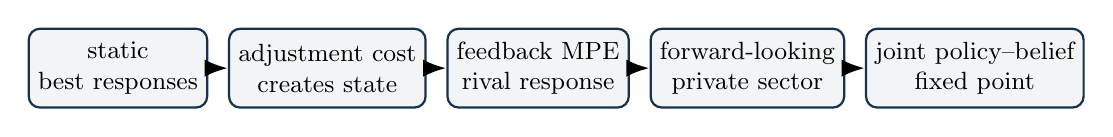
\begin{tikzpicture}[>=Latex,node distance=0.25cm,
  cbox/.style={draw=navy,thick,rounded corners,fill=softgray,
               align=center,minimum width=2.25cm,minimum height=1.0cm,
               font=\small}]
\node[cbox] (a) {static\\best responses};
\node[cbox,right=of a] (b) {adjustment cost\\creates state};
\node[cbox,right=of b] (c) {feedback MPE\\rival response};
\node[cbox,right=of c] (d) {forward-looking\\private sector};
\node[cbox,right=of d] (e) {joint policy--belief\\fixed point};
\draw[->,very thick] (a)--(b);
\draw[->,very thick] (b)--(c);
\draw[->,very thick] (c)--(d);
\draw[->,very thick] (d)--(e);
\end{tikzpicture}
\vspace{0.7cm}
\begin{columns}[T,onlytextwidth]
\column{0.47\textwidth}
\begin{block}{Question 1}
What structural terms make one authority react strongly to the other?
\end{block}
\begin{block}{Question 2}
When can current policy manipulate that future reaction?
\end{block}
\column{0.47\textwidth}
\begin{alertblock}{Question 3}
When do private expectations magnify the feedback without destroying
determinacy or stability?
\end{alertblock}
\end{columns}
\end{frame}

\section{1. Static interaction and leadership benchmark}

\begin{frame}{A minimal static policy environment}
Let the macroeconomic target vector be $y=(\pi,x)'$:
\begin{equation*}
\boxed{y=\bar y+D_Mm+D_Ff+e.}
\end{equation*}
For $i\in\{M,F\}$,
\begin{equation*}
L_i=(y-y_i^*)'W_i(y-y_i^*)+r_i a_i^2,
\qquad a_M=m,\quad a_F=f.
\end{equation*}
\begin{columns}[T,onlytextwidth]
\column{0.47\textwidth}
\begin{block}{Technology}
$D_M,D_F$ are signed policy-transmission vectors. Their direction determines
whether the instruments reinforce or offset one another in macro space.
\end{block}
\column{0.47\textwidth}
\begin{block}{Preferences}
$W_M,W_F$ encode mandate differences. $r_i>0$ is direct own-instrument
curvature and guarantees a finite desired action.
\end{block}
\end{columns}
\end{frame}

\begin{frame}{Static best responses}
The monetary first-order condition is
\begin{equation*}
D_M'W_M(y-y_M^*)+r_Mm=0.
\end{equation*}
Substitution for $y$ gives
\begin{align*}
m&=\alpha_M+R_{MF}f, &
R_{MF}&=-\frac{C_M}{H_M},\\
C_M&=D_M'W_MD_F, &
H_M&=r_M+D_M'W_MD_M.
\end{align*}
Similarly,
\begin{align*}
f&=\alpha_F+R_{FM}m, &
R_{FM}&=-\frac{C_F}{H_F},\\
C_F&=D_F'W_FD_M, &
H_F&=r_F+D_F'W_FD_F.
\end{align*}
\begin{alertblock}{Interpretation}
$C_i$ is cross-policy curvature under authority $i$'s mandate; $H_i$ is the
curvature of its own decision problem. A reaction is steep when
$|C_i|/H_i$ is large.
\end{alertblock}
\end{frame}

\begin{frame}{The static response product}
Solving the two best responses simultaneously gives
\begin{equation*}
\begin{bmatrix}m^N\\f^N\end{bmatrix}
=\frac{1}{1-\Gamma}
\begin{bmatrix}1&R_{MF}\\R_{FM}&1\end{bmatrix}
\begin{bmatrix}\alpha_M\\\alpha_F\end{bmatrix},
\qquad
\boxed{\Gamma=R_{MF}R_{FM}=\frac{C_MC_F}{H_MH_F}.}
\end{equation*}
\begin{columns}[T,onlytextwidth]
\column{0.47\textwidth}
\begin{block}{$\Gamma>0$: reciprocal reinforcement}
Reaction slopes have the same sign. As $\Gamma\to1^{-}$, small desired-policy
shifts produce large equilibrium actions.
\end{block}
\column{0.47\textwidth}
\begin{block}{$\Gamma<0$: reciprocal dampening}
Reaction slopes have opposite signs. The two responses counteract rather than
compound one another.
\end{block}
\end{columns}
\vfill
\centering Large mandate disagreement is insufficient unless it produces large
$|C_M|$ and $|C_F|$ relative to $H_M,H_F$.
\end{frame}

\begin{frame}{How shocks enter the static game}
The shock $e$ and target gaps enter $\alpha_M$ and $\alpha_F$; the structural
cross-curvatures determine the slopes.
\begin{columns}[T,onlytextwidth]
\column{0.47\textwidth}
\begin{block}{Demand-type disturbance}
Output and inflation move together.
\begin{itemize}
  \item Authorities may want stabilization in the same direction.
  \item Own instrument costs create an incentive to shift the burden.
  \item The realized game can resemble free riding.
\end{itemize}
\end{block}
\column{0.47\textwidth}
\begin{alertblock}{Cost-push disturbance}
Output and inflation move in opposite directions.
\begin{itemize}
  \item Mandate weights select different points on the trade-off.
  \item Each authority may offset the other's macroeconomic effect.
  \item The realized game can resemble an offset race.
\end{itemize}
\end{alertblock}
\end{columns}
\vfill
The shock also determines whether the equilibrium state loads heavily on the
direction in which strategic incentives operate.
\end{frame}

\begin{frame}{A one-period leadership benchmark}
Suppose the monetary authority chooses first and fiscal policy follows its best
response:
\begin{equation*}
f=BR_F(m)=\alpha_F+R_{FM}m.
\end{equation*}
The monetary leader solves
\begin{equation*}
\min_m L_M\bigl(m,BR_F(m)\bigr)
\end{equation*}
and recognizes
\begin{equation*}
\frac{dy}{dm}=D_M+D_FR_{FM}.
\end{equation*}
\begin{alertblock}{Role in the argument}
This benchmark reveals the value of manipulating the rival's reaction. It does
not explain where leadership comes from. The recursive MPE will endogenize the
same derivative through a payoff-relevant state.
\end{alertblock}
\end{frame}

\begin{frame}{Static parameters that make manipulation valuable}
The one-period leader advantage is large when:
\begin{enumerate}
  \item the follower slope $|R_{FM}|=|C_F|/H_F$ is large;
  \item the follower's action strongly affects the leader's targets,
        $\norm{D_F'W_M}$ is large;
  \item the leader can move its instrument cheaply enough, so $H_M$ is not too
        large;
  \item the shock/target gap makes the induced response valuable at the
        realized state.
\end{enumerate}
\begin{exampleblock}{Preview of the dynamic model}
Replace the imposed follower response $R_{FM}$ with the MPE derivative of
future fiscal policy with respect to today's monetary action.
\end{exampleblock}
\end{frame}

\section{2. Adjustment costs and feedback MPE}

\begin{frame}{Why dynamics are needed}
In a simultaneous policy game, neither authority can commit to a current move
before the other. Leadership requires a link from current policy to future
incentives.
\vspace{0.3cm}
\begin{equation*}
\boxed{\text{adjustment cost:}\qquad
\lambda_i(a_{i,t}-a_{i,t-1})^2.}
\end{equation*}
\begin{columns}[T,onlytextwidth]
\column{0.47\textwidth}
\begin{block}{Mechanical implication}
$a_{i,t}$ becomes the reference point for $a_{i,t+1}$. Current policy is now a
component of the next state.
\end{block}
\column{0.47\textwidth}
\begin{alertblock}{Strategic implication}
If the rival's feedback rule responds to that inherited position, current
policy changes future rival policy.
\end{alertblock}
\end{columns}
\end{frame}

\begin{frame}{A two-date feedback game}
Let $z_2$ contain macro states and the date-1 instruments. At date 2,
\begin{equation*}
m_2=k_{M,2}'z_2,qquad f_2=k_{F,2}'z_2.
\end{equation*}
At date 1, both authorities choose simultaneously and anticipate these
state-contingent date-2 rules:
\begin{align*}
V_{M,1}(z_1)&=\min_{m_1}\left\{\ell_{M,1}
            +\beta_MV_{M,2}(z_2)\right\},\\
V_{F,1}(z_1)&=\min_{f_1}\left\{\ell_{F,1}
            +\beta_FV_{F,2}(z_2)\right\}.
\end{align*}
\begin{alertblock}{Equilibrium concept}
Backward induction produces a finite-horizon Markov-perfect equilibrium:
strategies are optimal in every date-2 subgame and depend on the state inherited
from date 1.
\end{alertblock}
\end{frame}

\begin{frame}{The strategic-investment derivative}
Let the state evolve as
\begin{equation*}
z_{t+1}=Az_t+B_Mm_t+B_Ff_t.
\end{equation*}
Future fiscal policy responds to today's monetary action by
\begin{equation*}
\boxed{\frac{\partial f_{t+1}}{\partial m_t}=k_F'B_M.}
\end{equation*}
Decompose by state component $h$:
\begin{equation*}
k_F'B_M=\sum_h k_{Fh}B_{Mh}
=\underbrace{\sum_{h\in macro}k_{Fh}B_{Mh}}_{\text{macro-state channel}}
+\underbrace{k_{F,m^-}B_{M,m^-}}_{\text{inherited-policy channel}}.
\end{equation*}
\begin{alertblock}{Necessary condition}
Adjustment cost activates $m_t$ as $m_{t+1}^{-}$. Strategic investment still
vanishes if fiscal policy does not react to that state: $k_{F,m^-}=0$.
\end{alertblock}
\end{frame}

\begin{frame}{The rival-response term in the MPE first-order condition}
Schematically, monetary policy's continuation derivative is
\begin{equation*}
\frac{dV_{M,t+1}}{dm_t}
=\underbrace{V_{M,z}'B_M}_{\mathcal N_M:\ \text{own-state effect}}
+\underbrace{\mathcal H^M_{f,t+1}\,k_F'B_M}_{\mathcal S_M:\ \text{rival-response effect}},
\end{equation*}
where $\mathcal H^M_{f,t+1}$ is the monetary authority's shadow loss from a
marginal future fiscal action.
\vspace{0.3cm}
\begin{equation*}
\boxed{\mathcal S_M
=\beta_M\,(k_F'B_M)\,\mathcal H^M_{f,t+1}.}
\end{equation*}
\begin{alertblock}{Three factors}
The strategic term requires state exposure $B_M$, a future fiscal reaction
$k_F$, and a monetary payoff consequence $\mathcal H^M_f$.
\end{alertblock}
\end{frame}

\begin{frame}{Infinite-horizon recursive policy game}
Let
\begin{equation*}
z_t=(q_t,m_{t-1},f_{t-1},\varepsilon_t)'.
\end{equation*}
The Bellman equations are
\begin{align*}
V_M(z_t)&=\min_{m_t}\{\ell_M(z_t,m_t,f_t)+\beta_MV_M(z_{t+1})\},\\
V_F(z_t)&=\min_{f_t}\{\ell_F(z_t,m_t,f_t)+\beta_FV_F(z_{t+1})\}.
\end{align*}
Conjecture
\begin{equation*}
m_t=k_M'z_t,qquad f_t=k_F'z_t,qquad V_i(z_t)=z_t'P_iz_t.
\end{equation*}
\begin{block}{Stationary MPE}
Each rule is optimal given the rival's state-contingent rule, and the value
matrices reproduce themselves under the induced closed-loop transition.
\end{block}
\end{frame}

\begin{frame}{Coupled policy first-order conditions}
For stage-loss matrices $Q_M,Q_F$, simultaneous policy choices solve
\begin{equation*}\scriptsize
\begin{bmatrix}
Q^M_{mm}+\beta_MB_M'P_MB_M & Q^M_{mf}+\beta_MB_M'P_MB_F\\
Q^F_{fm}+\beta_FB_F'P_FB_M & Q^F_{ff}+\beta_FB_F'P_FB_F
\end{bmatrix}
\begin{bmatrix}m_t\\f_t\end{bmatrix}
=-
\begin{bmatrix}
Q^M_{mz}+\beta_MB_M'P_MA\\
Q^F_{fz}+\beta_FB_F'P_FA
\end{bmatrix}z_t.
\end{equation*}
This gives $m_t=k_M'z_t$ and $f_t=k_F'z_t$. With
$A_c=A+B_Mk_M'+B_Fk_F'$,
\begin{equation*}
P_i=C'Q_iC+\beta_iA_c'P_iA_c,qquad
C=\begin{bmatrix}I\\k_M'\\k_F'\end{bmatrix}.
\end{equation*}
\begin{alertblock}{Existence requirements}
The policy-response block must be nonsingular, value iterations must converge,
and $\rho(A_c)<1$ for a stable stationary solution.
\end{alertblock}
\end{frame}

\begin{frame}{Adjustment costs have two opposing effects}
Define the one-period persistence share
\begin{equation*}
p_i=\frac{\lambda_i}{D_i+\lambda_i},
\end{equation*}
where $D_i$ is non-adjustment own-action curvature.
\begin{columns}[T,onlytextwidth]
\column{0.30\textwidth}
\begin{block}{$p_i\approx0$}
The inherited instrument is almost irrelevant. There is little capacity to
bind the future.
\end{block}
\column{0.34\textwidth}
\begin{alertblock}{Intermediate $p_i$}
Current policy meaningfully shifts the future reference point while retaining
room to move today. Strategic investment can be large.
\end{alertblock}
\column{0.30\textwidth}
\begin{block}{$p_i\approx1$}
Policy is highly durable but current movement is prohibitively costly.
Commitment exists without usable investment capacity.
\end{block}
\end{columns}
\vfill
\centering The expected relationship between $\lambda_i$ and the strategic
effect is generally \key{hump-shaped}.
\end{frame}

\begin{frame}{Dynamic reciprocal response}
Define the two future cross-policy derivatives
\begin{equation*}
\varphi_{FM}=k_F'B_M,qquad
\varphi_{MF}=k_M'B_F,
\end{equation*}
and their product
\begin{equation*}
\boxed{\Omega=\varphi_{FM}\varphi_{MF}.}
\end{equation*}
\begin{columns}[T,onlytextwidth]
\column{0.47\textwidth}
\begin{block}{$\Omega>0$}
The intertemporal cross-responses reinforce one another. Bilateral attempts to
shape future positions can amplify.
\end{block}
\column{0.47\textwidth}
\begin{block}{$\Omega<0$}
The two intertemporal responses damp one another. One authority's investment
induces an offsetting future response.
\end{block}
\end{columns}
\vfill
$\Omega$ is a useful diagnostic, not a complete stability condition: the full
eigenvalues of $A_c$ also contain macro states and own persistence.
\end{frame}

\begin{frame}{Parameter set A: create a manipulable state}
For authority $i$ to invest strategically through its instrument, require
\begin{equation*}
\boxed{\lambda_i>0,qquad B_{i,a_i^-}\ne0,qquad
k_{j,a_i^-}\ne0.}
\end{equation*}
\begin{enumerate}
  \item $\lambda_i>0$ makes the inherited action payoff relevant.
  \item $B_{i,a_i^-}\ne0$ maps today's action into tomorrow's state.
  \item $k_{j,a_i^-}\ne0$ makes the rival respond to that inherited action.
\end{enumerate}
\begin{alertblock}{Not sufficient}
These restrictions produce a strategic derivative, but the derivative can be
economically negligible if the rival action barely affects authority $i$'s
loss or the relevant state is rarely activated.
\end{alertblock}
\end{frame}

\begin{frame}{Parameter set B: make the rival response steep}
The cross coefficient $k_{j,a_i^-}$ becomes large when the rival's FOC has
large cross-state curvature relative to own-action curvature:
\begin{equation*}
|k_{j,a_i^-}|\ \text{large when}\quad
\frac{|\text{effect of }a_i^-\text{ on rival target gradients}|}
{\text{rival own-action curvature}}
\quad\text{is large}.
\end{equation*}
This is favored by:
\begin{itemize}
  \item strong shared transmission of both instruments to output/inflation;
  \item mandate weights that make the inherited state important to the rival;
  \item low-to-moderate rival instrument penalty $r_j$;
  \item debt coefficients that transmit $a_i$ into a state the rival stabilizes;
  \item sufficiently persistent states, so the response is not immediately
        dissipated.
\end{itemize}
\end{frame}

\begin{frame}{Parameter set C: make the induced response valuable}
Even if $|k_j'B_i|$ is large, authority $i$ must care about the induced rival
action:
\begin{equation*}
\boxed{|\mathcal H^i_{j,t+1}|\ \text{large}.}
\end{equation*}
This requires:
\begin{itemize}
  \item the rival instrument to have a large effect on variables in $W_i$;
  \item a shock/target gap that gives those variables a large shadow value;
  \item mandate divergence that changes the desired policy mix, rather than
        merely rescaling both authorities' identical objective;
  \item limited direct substitutability through authority $i$'s own instrument;
  \item sufficient agency patience $\beta_i$.
\end{itemize}
\begin{alertblock}{State dependence}
LQ feedback coefficients are constant, but the realized strategic FOC wedge is
linear in the state. A shock orthogonal to the relevant shadow-value direction
can produce a small effect even with steep rules.
\end{alertblock}
\end{frame}

\section{3. Add the forward-looking NK private sector}

\begin{frame}{The forward-looking macro block}
Let $x_t$ be the output gap, $\pi_t$ inflation, $m_t$ monetary tightening, and
$f_t$ fiscal expansion:
\begin{align*}
x_t&=\E_tx_{t+1}
-\sigma\bigl(m_t-\E_t\pi_{t+1}\bigr)+\psi f_t+d_t,\\
\pi_t&=\beta_p\E_t\pi_{t+1}+\kappa x_t+u_t,\\
b_{t+1}&=\rho_bb_t+\chi_mm_t+\chi_ff_t-\chi_\pi\pi_t.
\end{align*}
\begin{columns}[T,onlytextwidth]
\column{0.47\textwidth}
\begin{block}{Direct policy transmission}
$\sigma,\psi,\kappa,$ and the debt coefficients determine how current
instruments alter current targets and the next macro state.
\end{block}
\column{0.47\textwidth}
\begin{alertblock}{Expectations transmission}
Expected future output and inflation bring anticipated future policy responses
into current private decisions.
\end{alertblock}
\end{columns}
\end{frame}

\begin{frame}{Timing in the forward-looking MPE}
\centering
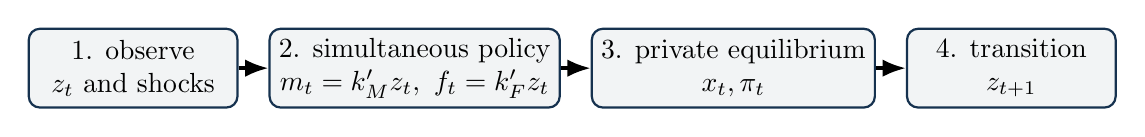
\begin{tikzpicture}[>=Latex,node distance=0.38cm,
  tbox/.style={draw=navy,thick,rounded corners,fill=softgray,
               align=center,minimum height=1.0cm,minimum width=2.65cm}]
\node[tbox] (s) {1. observe\\$z_t$ and shocks};
\node[tbox,right=of s] (p) {2. simultaneous policy\\$m_t=k_M'z_t,\ f_t=k_F'z_t$};
\node[tbox,right=of p] (y) {3. private equilibrium\\$x_t,\pi_t$};
\node[tbox,right=of y] (n) {4. transition\\$z_{t+1}$};
\draw[->,very thick] (s)--(p);
\draw[->,very thick] (p)--(y);
\draw[->,very thick] (y)--(n);
\end{tikzpicture}
\vspace{0.7cm}
\begin{itemize}
  \item Private agents observe current instruments and know the stationary MPE
        rules that will be used in future states.
  \item Each authority understands current private responses and the law of
        motion, but cannot bind future discretion beyond the states it creates.
  \item No Taylor rule or fiscal rule is imposed exogenously.
\end{itemize}
\end{frame}

\begin{frame}{Private forecasting rule}
Let $y_t=(x_t,\pi_t)'$ and $q_t=(z_t',m_t,f_t)'$. Before imposing private
equilibrium,
\begin{equation*}
z_{t+1}=Nq_t+Ey_t.
\end{equation*}
Private agents conjecture the stationary forecast
\begin{equation*}
\boxed{\E_ty_{t+1}=Gz_{t+1}.}
\end{equation*}
\begin{block}{Meaning of $G$}
$G$ maps tomorrow's predetermined state into tomorrow's equilibrium output and
inflation. Because future policy rules depend on that state, $G$ embeds expected
future monetary and fiscal behaviour.
\end{block}
\begin{alertblock}{New equilibrium loop}
Policy rules depend on private transmission generated by $G$, while $G$ must be
validated by those same policy rules.
\end{alertblock}
\end{frame}

\begin{frame}{Reduce the private block conditional on $G$}
Collect the IS and Phillips curves as
\begin{equation*}
Ly_t=Dq_t+HGz_{t+1},qquad
L=\begin{bmatrix}1&0\\-\kappa&1\end{bmatrix},\quad
H=\begin{bmatrix}1&\sigma\\0&\beta_p\end{bmatrix}.
\end{equation*}
Using $z_{t+1}=Nq_t+Ey_t$,
\begin{align*}
M(G)y_t&=[D+HGN]q_t,\\
M(G)&=L-HGE,\\
y_t&=O(G)q_t,\qquad O(G)=M(G)^{-1}[D+HGN].
\end{align*}
\begin{alertblock}{Within-period solvability}
$M(G)$ must be nonsingular. Its smallest singular value controls how strongly
beliefs about the future feed back into current private outcomes.
\end{alertblock}
\end{frame}

\begin{frame}{The policy game conditional on private beliefs}
The reduced transition is
\begin{equation*}
z_{t+1}=A(G)z_t+B_M(G)m_t+B_F(G)f_t.
\end{equation*}
The target equations imply belief-dependent stage-loss matrices $Q_i(G)$.
Conditional on $G$, solve exactly the same coupled MPE system:
\begin{equation*}
(k_M(G),k_F(G),P_M(G),P_F(G))
=\operatorname{MPE}\bigl(A(G),B_M(G),B_F(G),Q_M(G),Q_F(G)\bigr).
\end{equation*}
\begin{block}{Analytical continuity}
The forward-looking NK model does not replace the recursive strategic-
investment game. It changes the matrices through which states and policies
affect current targets and future values.
\end{block}
\end{frame}

\begin{frame}{Close the rational-expectations MPE}
Partition $O(G)=(O_z,O_m,O_f)$. Given the solved policy rules, the actual
private outcome rule is
\begin{equation*}
y_t=\left[O_z(G)+O_m(G)k_M(G)'+O_f(G)k_F(G)'\right]z_t.
\end{equation*}
Rational expectations require
\begin{equation*}
\boxed{G=\Phi(G)
=O_z(G)+O_m(G)k_M(G)'+O_f(G)k_F(G)'.}
\end{equation*}
\begin{alertblock}{Stationary rational-expectations MPE}
A solution is a fixed point in private beliefs, agency feedback rules, and
agency value matrices, with a stable closed-loop state transition.
\end{alertblock}
\end{frame}

\begin{frame}{The forward-looking amplification operator}
The direct sensitivity of current private outcomes to a change in expected
future outcomes is governed by
\begin{equation*}
\boxed{\mathcal A_E(G)=M(G)^{-1}H=[L-HGE]^{-1}H.}
\end{equation*}
Large amplification is associated with
\begin{equation*}
\norm{\mathcal A_E(G)}\ \text{large}
\quad\Longleftrightarrow\quad
\sigma_{\min}(L-HGE)\ \text{small}.
\end{equation*}
\begin{columns}[T,onlytextwidth]
\column{0.47\textwidth}
\begin{block}{Magnifying parameters}
High $\beta_p$, strong intertemporal demand sensitivity $\sigma$, a steep
Phillips curve $\kappa$, and state-contingent future policy can strengthen the
expectations loop.
\end{block}
\column{0.47\textwidth}
\begin{alertblock}{Boundary}
If $M(G)$ becomes singular or the full fixed point loses stability, the object
is not a robust strategic equilibrium; it is a determinacy problem.
\end{alertblock}
\end{columns}
\end{frame}

\begin{frame}{Forward-looking strategic-investment product}
The inherited-policy component of authority $i$'s strategic FOC can be written
schematically as
\begin{equation*}
\boxed{
\mathcal S_i^{policy}
=\beta_i
\underbrace{B_{i,a_i^-}}_{\text{state creation}}
\underbrace{k_{j,a_i^-}}_{\text{rival response}}
\underbrace{\mathcal H^i_{j}}_{\text{payoff exposure}},}
\end{equation*}
with $\mathcal H^i_j$ itself affected by
\begin{equation*}
\underbrace{M(G)^{-1}H}_{\text{private expectations transmission}}
\quad\text{and}\quad
\underbrace{P_i}_{\text{discounted future shadow values}}.
\end{equation*}
\begin{alertblock}{Central result}
Forward-looking behaviour is a multiplier on the economic response chain. If
state creation, rival response, or payoff exposure is zero, expectations alone
cannot generate strategic investment.
\end{alertblock}
\end{frame}

\section{4. Parameter regions for a large strategic effect}

\begin{frame}{A useful magnitude bound}
By submultiplicativity,
\begin{equation*}
|\mathcal S_i|
\le
\beta_i\norm{B_i}\norm{k_j}\,|\mathcal H^i_j|.
\end{equation*}
In the forward-looking model, a corresponding bound is
\begin{equation*}
|\mathcal H^i_j|
\lesssim
c_{0i}+c_{1i}\norm{M(G)^{-1}H}\norm{P_i},
\end{equation*}
for constants collecting mandate and transmission terms.
\begin{block}{Four multiplicative margins}
\begin{enumerate}
  \item policy-to-state exposure $\norm{B_i}$;
  \item rival rule sensitivity $\norm{k_j}$ in the relevant direction;
  \item private expectations amplification $\norm{M^{-1}H}$;
  \item discounted payoff shadow value $\norm{P_i}$.
\end{enumerate}
\end{block}
\end{frame}

\begin{frame}{Necessary restrictions for a nonzero effect}
For the narrow inherited-policy channel of authority $i$,
\begin{equation*}
\boxed{
\lambda_i>0,quad
B_{i,a_i^-}\ne0,quad
k_{j,a_i^-}\ne0,quad
\mathcal H^i_j\ne0,quad
z_t\ne0\text{ in the relevant direction}.}
\end{equation*}
If any factor is zero:
\begin{itemize}
  \item no adjustment cost $\Rightarrow$ no payoff-relevant inherited action;
  \item no state mapping $\Rightarrow$ current policy does not survive;
  \item no rival reaction $\Rightarrow$ only own smoothing remains;
  \item no payoff exposure $\Rightarrow$ the induced rival action is irrelevant;
  \item no state loading $\Rightarrow$ the mechanism exists in the rule but is
        not activated by the disturbance.
\end{itemize}
\end{frame}

\begin{frame}{Sufficient ingredients for an economically large effect}
An economically large and robust effect requires the intersection of:
\begin{enumerate}
  \item \key{interior commitment capacity}: $p_i$ high enough to create
        persistence, but below the near-immobility region;
  \item \key{strong cross curvature}: $|C_j|/H_j$ or its dynamic analogue is
        large;
  \item \key{large payoff spillover}: the rival instrument moves targets heavily
        weighted by authority $i$;
  \item \key{patience and durable states}: $\beta_i$ and relevant persistence
        parameters are high;
  \item \key{strong but determinate expectations}: $\norm{M^{-1}H}$ is large
        while $M$ remains nonsingular;
  \item \key{closed-loop stability}: $\rho(A_c)<1$ with a nontrivial margin.
\end{enumerate}
\begin{alertblock}{Intersection, not addition}
One large parameter cannot compensate for a zero elsewhere in the response
chain.
\end{alertblock}
\end{frame}

\begin{frame}{Analytical phase diagram}
\centering
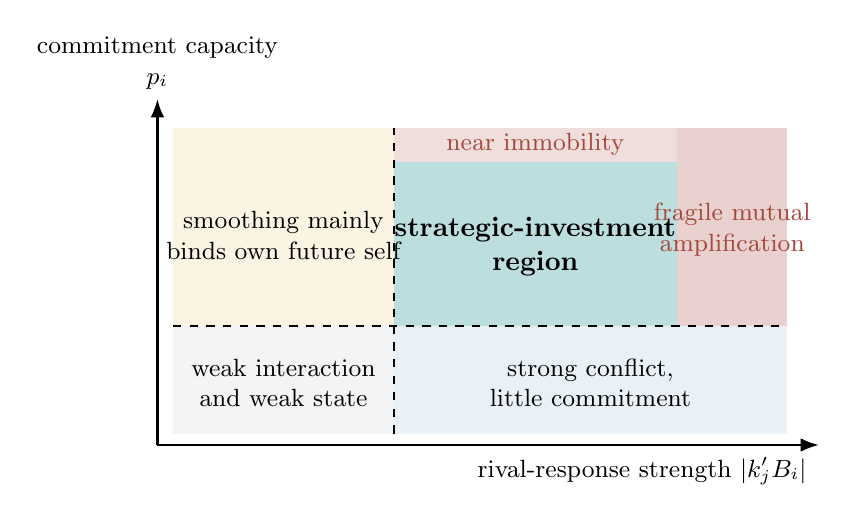
\begin{tikzpicture}[x=1.0cm,y=0.72cm,>=Latex,font=\small]
  \draw[->,thick] (0,0)--(8.4,0)
    node[below left=1pt]{rival-response strength $|k_j'B_i|$};
  \draw[->,thick] (0,0)--(0,6.1) node[above,align=center]{commitment capacity\\$p_i$};
  \fill[softgray] (0.2,0.2) rectangle (3.0,2.1);
  \fill[lightblue] (3.0,0.2) rectangle (8.0,2.1);
  \fill[lightgold] (0.2,2.1) rectangle (3.0,5.6);
  \fill[teal!28] (3.0,2.1) rectangle (6.6,5.0);
  \fill[brick!25] (6.6,2.1) rectangle (8.0,5.6);
  \fill[brick!18] (3.0,5.0) rectangle (6.6,5.6);
  \node[align=center] at (1.6,1.1) {weak interaction\\and weak state};
  \node[align=center] at (5.5,1.1) {strong conflict,\\little commitment};
  \node[align=center] at (1.6,3.7) {smoothing mainly\\binds own future self};
  \node[align=center,font=\bfseries] at (4.8,3.5) {strategic-investment\\region};
  \node[align=center,text=brick] at (7.3,3.8) {fragile mutual\\amplification};
  \node[align=center,text=brick] at (4.8,5.3) {near immobility};
  \draw[dashed,thick] (3.0,0.2)--(3.0,5.6);
  \draw[dashed,thick] (0.2,2.1)--(8.0,2.1);
\end{tikzpicture}
\vfill
\centering A large robust effect lies away from both zero-persistence and
near-immobility boundaries, with a strong but stable rival response.
\end{frame}

\begin{frame}{How each parameter enters}
\scriptsize
\begin{tabular}{@{}>{\raggedright\arraybackslash}p{0.16\textwidth}
                    >{\raggedright\arraybackslash}p{0.34\textwidth}
                    >{\raggedright\arraybackslash}p{0.40\textwidth}@{}}
\toprule
Parameter & Direct channel & Condition for a larger strategic effect \\
\midrule
$\lambda_i$ & creates inherited-policy state & interior range: durable but still movable \\
$r_i$ & own-action curvature & lower $r_i$ steepens responses, subject to convexity/stability \\
$\sigma,\psi$ & direct policy transmission to demand & raises cross curvature and payoff exposure if both agencies care about induced targets \\
$\kappa$ & output-to-inflation pass-through & raises cross-target effects when inflation has shadow value \\
$\beta_p$ & expected-inflation transmission & raises $\norm{M^{-1}H}$ only if the policy-belief loop remains determinate \\
$\rho_b,\chi$ & durability and policy exposure of debt & useful when the rival responds to debt and debt affects the first authority's loss \\
$\beta_i$ & policy patience & raises the weight on the future rival response \\
$W_M,W_F$ & mandate curvature & must steepen cross-responses; difference alone is insufficient \\
shock persistence & duration of shadow-value state & raises importance when the shock loads on the strategic direction \\
\bottomrule
\end{tabular}
\end{frame}

\begin{frame}{Strategic complementarity and equilibrium multiplicity}
The rational-expectations map is
\begin{equation*}
G=\Phi(G).
\end{equation*}
Local uniqueness is threatened when
\begin{equation*}
\rho\bigl(D\Phi(G^*)\bigr)\approx1,
\end{equation*}
because a change in expected future outcomes induces policy and private-sector
responses that almost validate the original change.
\begin{columns}[T,onlytextwidth]
\column{0.47\textwidth}
\begin{block}{Parameters pushing toward complementarity}
High private expectations transmission, persistent states, steep policy rules,
low instrument curvature, and mutually reinforcing mandates.
\end{block}
\column{0.47\textwidth}
\begin{alertblock}{What must still be checked}
Multiple fixed points are possible, not automatic. One must establish fixed-
point existence, local Jacobian properties, and closed-loop stability for each
candidate equilibrium.
\end{alertblock}
\end{columns}
\end{frame}

\begin{frame}{Do not measure strategic importance with one statistic}
Use three complementary diagnostics:
\begin{align*}
\text{absolute wedge:}\quad & |\mathcal S_i|,\\
\text{bounded FOC share:}\quad &
\frac{|\mathcal S_i|}{|\mathcal S_i|+|\mathcal N_i|},\\
\text{equilibrium displacement:}\quad &
\norm{K^{\lambda}-K^{0}}\quad\text{or}\quad
\norm{a_t^{\lambda}-a_t^{0}}.
\end{align*}
\begin{alertblock}{Cancellation problem}
A strategic share can be close to one because the nonstrategic continuation
term is close to zero, even when the absolute wedge and policy displacement are
tiny. Stability margins must be reported alongside all three diagnostics.
\end{alertblock}
\end{frame}

\begin{frame}{A disciplined analytical experiment}
Map the model entirely in dimensionless coordinates:
\begin{enumerate}
  \item persistence share $p_i=\lambda_i/(D_i+\lambda_i)$;
  \item static response product $\Gamma=C_MC_F/(H_MH_F)$;
  \item dynamic reciprocal response $\Omega=(k_F'B_M)(k_M'B_F)$;
  \item expectations gain $\mathcal E=\norm{M(G)^{-1}H}$;
  \item stability margin $1-\rho(A_c)$;
  \item belief fixed-point margin $1-\rho(D\Phi(G^*))$.
\end{enumerate}
\begin{exampleblock}{Goal}
Identify regions where absolute wedges, equilibrium displacement, and stability
jointly indicate meaningful strategic investment. The axes themselves are
structural mechanisms, not country-specific values.
\end{exampleblock}
\end{frame}

\section{Conclusions}

\begin{frame}{What generates a large strategic effect?}
\begin{equation*}
\boxed{
\begin{aligned}
\text{large effect}
&=\text{state creation}\times\text{rival response}\times\text{payoff exposure}\\
&\quad\times\text{expectations gain}\times\text{patience}.
\end{aligned}}
\end{equation*}
\begin{enumerate}
  \item Adjustment cost is necessary for the narrow inherited-policy channel,
        but is not itself the strategic effect.
  \item The decisive object is the rival's MPE response to the state created by
        current policy.
  \item Forward-looking private behaviour transmits that future response into
        current output and inflation.
  \item High persistence and strong expectations can also produce immobility,
        instability, or indeterminacy.
  \item Robust importance requires a large absolute wedge, visible equilibrium
        displacement, and safe stability margins.
\end{enumerate}
\end{frame}

\begin{frame}{Next analytical steps}
\begin{enumerate}
  \item Derive closed-form $k_{j,a_i^-}$ in a reduced scalar version of the NK
        game.
  \item Characterize signs of $\Gamma$ and $\Omega$ for demand versus cost-push
        disturbances and alternative mandate weights.
  \item Compute $D\Phi(G^*)$ to locate rational-expectations complementarity and
        possible multiple MPE branches.
  \item Map $(p_i,\Gamma,\mathcal E)$ jointly with both stability margins.
  \item Derive boundary cases that separate negligible, large, and unstable
        strategic effects without assigning country-specific values.
\end{enumerate}
\vfill
\centering\large\key{The central task is to characterize the mechanism,
its sign, and its stable parameter region.}
\end{frame}

\begin{frame}{Selected references}
\footnotesize
\begin{itemize}
  \item Clarida, Gal\'i and Gertler (1999), ``The Science of Monetary Policy.''
  \item Debelle and Fischer (1994), ``How Independent Should a Central Bank Be?''
  \item Dixit and Lambertini (2003), ``Interactions of Commitment and
        Discretion in Monetary and Fiscal Policies.''
  \item Jun and Vives (2004), ``Strategic Incentives in Dynamic Duopoly.''
  \item Petkov (2004), ``Delegated Management in Dynamic Oligopolies.''
  \item Muscatelli, Tirelli and Trecroci (2004), ``Fiscal and Monetary Policy
        Interactions.''
  \item Kirsanova and Yates (2025), ``Multiple Equilibria in the Absence of
        Commitment.''
\end{itemize}
\vfill
\centering\large\key{Questions and discussion}
\end{frame}

\appendix
\section{Analytical backup}

\begin{frame}{Backup: static Nash derivation}
For authority $M$,
\begin{align*}
L_M&=(\bar y+D_Mm+D_Ff+e-y_M^*)'W_M
     (\bar y+D_Mm+D_Ff+e-y_M^*)+r_Mm^2,\\
0&=D_M'W_M(\bar y+D_Mm+D_Ff+e-y_M^*)+r_Mm,\\
m&=-\frac{D_M'W_M(\bar y+e-y_M^*)}{H_M}
   -\frac{C_M}{H_M}f.
\end{align*}
Thus
\begin{equation*}
\alpha_M=-\frac{D_M'W_M(\bar y+e-y_M^*)}{H_M},
\qquad R_{MF}=-\frac{C_M}{H_M}.
\end{equation*}
The fiscal expression follows symmetrically.
\end{frame}

\begin{frame}{Backup: social welfare and coordination}
Let true social loss be
\begin{equation*}
L_S=(y-y_S^*)'W_S(y-y_S^*)+r_M^Sm^2+r_F^Sf^2.
\end{equation*}
The cooperative static allocation solves
\begin{equation*}
\begin{bmatrix}
D_M'W_SD_M+r_M^S&D_M'W_SD_F\\
D_F'W_SD_M&D_F'W_SD_F+r_F^S
\end{bmatrix}
\begin{bmatrix}m\\f\end{bmatrix}
=-
\begin{bmatrix}D_M'W_S\\D_F'W_S\end{bmatrix}
(\bar y+e-y_S^*).
\end{equation*}
\begin{alertblock}{Distinction}
Coordination changes which objective is minimized. Commitment capacity changes
the state transition and intertemporal feasible set. They are not substitutes.
\end{alertblock}
\end{frame}

\begin{frame}{Backup: Riccati update}
Let
\begin{equation*}
K=\begin{bmatrix}k_M'\\k_F'\end{bmatrix},qquad
C=\begin{bmatrix}I\\K\end{bmatrix},qquad
A_c=A+[B_M\ B_F]K.
\end{equation*}
For each authority,
\begin{equation*}
P_i=C'Q_iC+\beta_iA_c'P_iA_c.
\end{equation*}
A stationary solution requires:
\begin{itemize}
  \item a nonsingular simultaneous policy response block;
  \item finite positive-semidefinite value matrices;
  \item convergence of the coupled policy/value iteration;
  \item $\rho(A_c)<1$.
\end{itemize}
\end{frame}

\begin{frame}{Backup: broad versus narrow strategic channels}
For monetary policy,
\begin{equation*}
k_F'B_M
=k_{F,b}B_{M,b}
+k_{F,m^-}B_{M,m^-}
+k_{F,f^-}B_{M,f^-}
+k_{F,d}B_{M,d}
+k_{F,u}B_{M,u}.
\end{equation*}
\begin{itemize}
  \item $k_{F,b}B_{M,b}$: strategic response through public debt;
  \item $k_{F,m^-}B_{M,m^-}$: monetary inherited-policy investment;
  \item other terms: shock or institutional-state channels.
\end{itemize}
\begin{alertblock}{Interpretation}
Strategic interaction can exist without adjustment costs through persistent
macro states. The Petkov mechanism is the narrower inherited-policy term.
\end{alertblock}
\end{frame}

\begin{frame}{Backup: fixed-point Jacobian}
At a rational-expectations equilibrium $G^*=\Phi(G^*)$, a local perturbation
satisfies
\begin{equation*}
\operatorname{vec}(\Delta G_{n+1})
\approx D\Phi(G^*)\operatorname{vec}(\Delta G_n).
\end{equation*}
\begin{itemize}
  \item $\rho(D\Phi)<1$: locally contractive belief iteration;
  \item $\rho(D\Phi)\approx1$: strong expectations complementarity and slow
        convergence;
  \item $\rho(D\Phi)>1$: the simple iteration is unstable and additional fixed
        points or equilibrium-selection issues become plausible.
\end{itemize}
\begin{alertblock}{Caution}
Numerical convergence of one damped algorithm is not a global uniqueness proof.
\end{alertblock}
\end{frame}

\end{document}
